\section{Learning to Optimally Segment Point Clouds}\label{header-n863}

\emph{IEEE ROBOTICS AND AUTOMATION LETTERS, VOL. 5, NO. 2, APRIL 2020}
{[}28{]}

\subsection{Introduction}\label{header-n865}

This letter focuses on the application of autonomous vehicles.
Perception for autonomous robots presents a series of challenges. First,
the right representation of the 3D data obtained by a LiDAR sensor still
remains an open question. Secondly, contemporary approaches to object
detection and scene understanding tend to be closed-world, where the
task is predicting 1-of-N possible labels. Finally, practical autonomous
robotics makes heavy use of perceptual priors in the forms of geometric
maps and assumptions on LiDAR geometry. In this work, the authors focus
on the problem of class-agnostic instance segmentation of LiDAR point
clouds in an open-world setting.

\begin{figure}[h!]
\centering
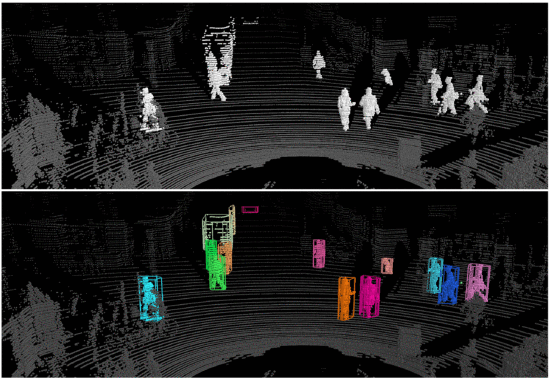
\includegraphics[width=0.7\linewidth]{images/pointcloudseg.png}
\caption{The class-agnostic instance-level segmentation over all foreground points performed by the proposed method }
\end{figure}

They carefully mix graph-theoretic algorithms with data-driven learning.
While data-driven learning is widely used due to its performance, it is
difficult to guarantee good results when processing out-of-sample data
from an open world. The proposed method searches over an exponentially
large space of possible segmentations and returns the one most similar
to the data-driven point-based model of ``objectness". First, the search
is restricted into a subset of segmentations that are consistent with a
hierarchical grouping of a point cloud sweep. Such hierarchical groups
can be readily produced with agglomerative clustering or hierarchical
graph-based algorithms. Since that a segmentation algorithm can produce
an exponentially-large set of segmentations, the authors introduce
efficient algorithms that search over a space of tree-consistent
segmentations and return the one that maximizes a global segmentation
score.

\subsection{Proposed approach}\label{header-n869}

For 3D object point segmentation, the input is a 3D point cloud, which
contains an \emph{unknown} number of objects. The goal is to produce a
point segmentation, in which every segment contains points from one and
only one object.

\subsubsection{Definitions}\label{header-n871}

A \emph{global segmentation} $P_X$ is a partition of a set of points
$X$ into subsets of points $C_i$ (called local segment), i.e
$P_X = \{C_i\}_{i = 1}^{M}$, where $M$ denotes the number of
segments and $C_i \subset X$. Importantly, every point exists in one
and only one segment.

The concept of \emph{tree-consistent segmentation} is defined as
follows. The set of all possible global segmentations on $X$ is
defined as $S_X$. Without constraints, the size of $S_X$ is
exponential but in practice the authors reduce the number of candidates
by enforcing geometric constraints. All points are grouped
hierarchically into a tree structure $T_X$. Now, the tree-consistent
segmentation is $S_{X,T}$ and contains all possible segmentation
defined by the tree $T$. The following figure illustrates the
relationship between $S_X$ and $S_{X,T}$.

\begin{figure}[h!]
\centering
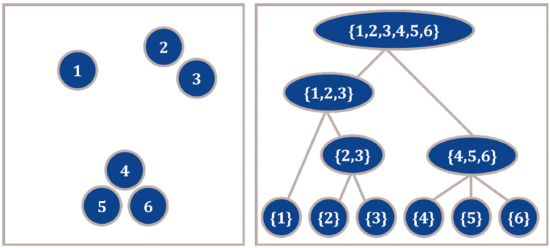
\includegraphics[width=0.7\linewidth]{images/treesegment.png}
\caption{Tree-consistent segmentation}
\end{figure}

Any tree-consistent segmentation from corresponds to a vertex cut set of
the tree $T$, i.e. a set of tree nodes, which satisfy the following
constraints:

\begin{itemize}
\item
  for each node in the vertex cut, its ancestor and itself cannot both
  be in the cut and
\item
  each leaf node must have itself or its ancestor in the cut. 
\end{itemize}

The \emph{segment score} is defined as a function $f(C, \theta)$,
where $C$ is the segment and $\theta$ are the function parameters.
$f$ predicts a given segment's ``objectness" and can be implemented by
a PointNet++, where $\theta$ are the network's weights.

The \emph{segmentation score} is calculated as the aggregation of the
score of all segments in a global segmentation $P_X$. Formally, given
a global segmentation $P_X = \{Ci\}^{M}_{i=1}$, its score is
$F(P_X; \theta) : PX→ [0, 1]$ by aggregating over local objectness of
all its segments.

\subsubsection{Worst-case segmentation}\label{header-n884}

The \emph{worst-case segmentation} score of a global segmentation is the
worst objectness among its local segments:

$ F_{\min }(P_X; \theta) = \min _i{f(C_i; \theta)}, i\in {1 \ldots M}.$

Now, the optimal worst-case segmentation is

$ P_{X,\min }^* = \mathop{\operatorname{argmax}}\limits_{P_X\in S_{X,T}} {F_{\min } (P_X; \theta)} $.

It turns out the problem of finding optimal worst-case segmentation has
optimal substructure, allowing us to find the global optimum efficiently
with dynamic programming (see the following figure).

\begin{figure}[h!]
\centering
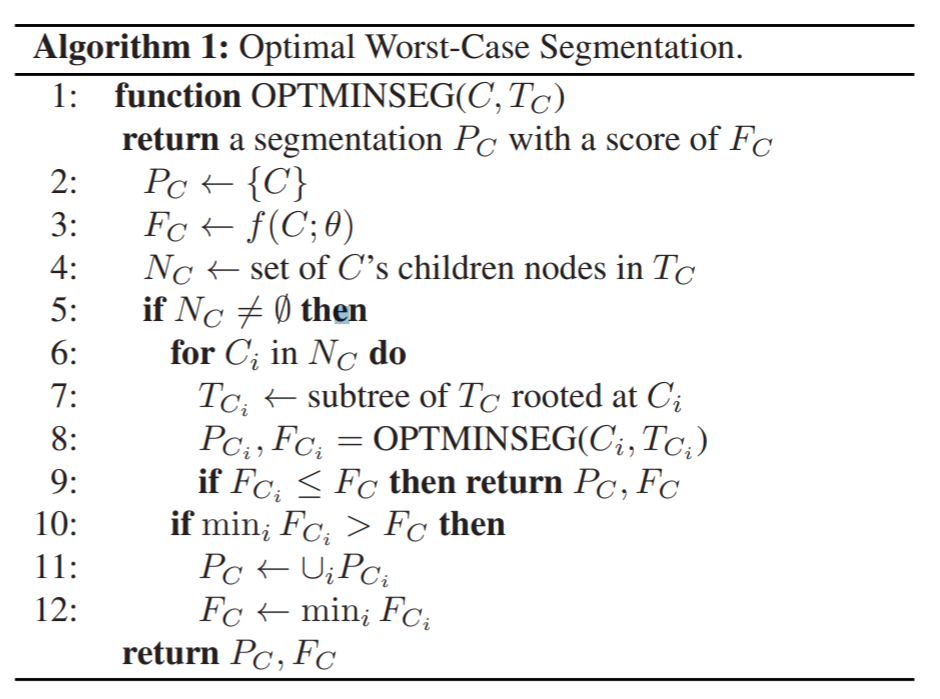
\includegraphics[width=0.8\linewidth]{images/worstcaseseg.png}
\caption{Optimal worst case segmentation}
\end{figure}

The algorithm starts from the root node $X$ and chooses between a
coarse segmentation and a fine one. The fine segmentation will be the
union of all $X$`s children's optimal worst-case segmentation, which
can be computed recursively. The algorithm would first traverse down to
the leaf nodes, representing the finest segmentation. Then it will make
its way up, during which it finalizes optimal segmentation for each
intermediate node by making local coarse vs. fine decisions. Eventually,
it returns to the root node and produces an optimal worst-case global
segmentation. This algorithm might not visit all nodes. Instead, it
skips a sub-trees whenever one sub-tree exhibits a lower score. The
algorithm's complexity is linear in $N$ despite the fact that the
search space is exponential in $N$.

\subsubsection{Average-case segmentation}\label{header-n892}

Average-case segmentation score of a global segmentation is the average
objectness among its local segments:
\newline
$ F_{\operatorname{avg}{}}(P_X; \theta) = \frac{1}{M} \sum _{i=1}^M f(C_i; \theta).$
\newline
$P_{X,\operatorname{avg}{}}^*$ can be defined as \emph{optimal
average-case segmentation} if
\newline
$ P_{X,\operatorname{avg}{}}^* = \mathop{\operatorname{argmax}}\limits_{P_X\in S_{X,T}} {F_{\operatorname{avg}{}} (P_X; \theta)}. $
\newline
It is important to specify that the problem of finding the optimal
average-case segmentation does not have optimal substructure, unlike
worst-case segmentation.

\subsubsection{Learning the Objectness Function}\label{header-n898}

Until now, the segmentation algorithms have been discussed under the
assumption that the objectness function $f(C; \theta)$ is defined (it
predicts an objectness score for a given point cloud). First of all, the
ground-truth function must be defined. Suppose to have the ground truth
segmentation $P^{gt} = \{C_1^{gt},...,C_L^{gt}\}$. To define the
target objectness of a segment, we have to consider that 3D sensors
(e.g. LiDAR) tend to produce denser points near the sensor. In
consequence, the objectness will be heavily influenced by the
partitioning of points closer to the sensor. A segment objectness
function of a segment is the largest point between itself and any ground
truth segment:
\newline
$ Objectness(C, P^{gt}) = \max _{l=1,\ldots,L} \frac{\sum _{x \in C \cap C^{gt}_l} x^T x }{\sum _{x \in C \cup C^{gt}_l} x^T x }, $
\newline
where $x^T x$ represents the squared distance of a point $x$ to
sensor origin. The authors train a PointNet++ model for learning the
objectness function. Each segment is re-sampled to 1024 points.

\subsubsection{Building tree hierarchies}\label{header-n902}

This section explains how to build a tree structure given a set of
points $X$. One natural approach is agglomerative clustering, merging
points in classes according to their spatial features. This approach
tends to create tree hierarchies with very fine granularity, e.g. one
node may differ from another with only one point of difference. In this
work, the authors propose a method which builds a coarser tree whose
leaf nodes are segments (rather than individual points) and adjacent
nodes should differ from each other much more. To build such a tree,
Euclidean Clustering algorithm is used recursively in a top-down fashion
with a list of decreasing $\epsilon$. In the beginning, the algorithm
is run with the largest $\epsilon$ value, defining the most coarse
connected components. Then, the procedure is repeated a smaller
$\epsilon$ within each connected component. This produces a
multiple-tree top-down hierarchy.

\subsection{Experiments}\label{header-n904}

For evaluation, the authors repurpose the KITTI object detection
benchmark for point cloud segmentation, following the setup in {[}30{]}.
The ground truth segmentation is composed of a series of point segments
marked with a bounding box. All the background points (those outside the
bounding box) are removed. To evaluate the performance are considered
two metrics: the \emph{under-segmentation error} $U$ and the
\emph{over-segmentation error} $O$, defined as follows:
\newline
$ U = \frac{1}{L} \sum _{l=1}^L \mathbf {1} \left(\frac{|C_{i^*} \cap C_l^{gt}|}{|C_{i^*}|} < \tau _U\right) \\ O = \frac{1}{L} \sum _{l=1}^L \mathbf {1} \left(\frac{|C_{i^*} \cap C_l^{gt}|}{|C_l^{gt}|} < \tau _O\right)$
\newline
with
\newline
$ i^* = \operatorname{argmax}_{i=1}^M{|C_i \cap C^{gt}_l|}$
\newline
and $\tau _U, \tau _O$ as constant thresholds, set to
$\frac{2}{3}, 1$.
\newline
The Euclidean clustering algorithm is applied with an
$\epsilon \in \{2 m, 1 m, 0.5 m, 0.25 m\}$. The authors include it as
a baseline to find better solutions. As baselines, other
state-of-the-art 3D detectors are included: AVOD, PointPillars,
PointRCNN, and SECOND. Since these detectors output class-specific
bounding box detection, the authors simply ignore the class label to
produce class-agnostic segmentations. In addition, the authors include
for evaluation modified versions of the proposed baselines, in order to
improve their performance. A much better approach, called
\emph{\{Detector\}++} (e.g. AVOD++ etc.), check if the leftover segments
can be included in an existing detection segment. Another approach,
SECOND++, consists of re-train and re-evaluate the best baseline, i.e.
SECOND, with background removal. These baselines are marked with ``+ BG
Removal". In addition, the authors discover that, by extending the
SECOND's detection range from 50 m to 80 m, the SECOND's performance is
significantly improved. The affected baselines are marked with ``+ Ext.
Range". Finally, they re-train and re-evaluate SECOND on all 8 classes.
The new baselines are labeled as ``SECOND++(8)", while the off-the-shelf
SECOND baselines are labeled as ``SECOND++(4)". The following figure
resumes the results obtained.

\begin{figure}[h!]
\centering
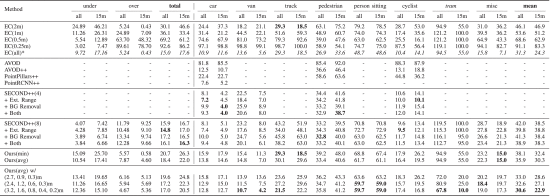
\includegraphics[width=1\linewidth]{images/segmentationerrors.png}
\caption{Segmentation errors on the proposed method (*Ours*) and the baselines}
\end{figure}

The table shows that the average-case segmentation, \emph{Ours(avg)},
consistently outperforms the optimal worst-case segmentation
\emph{Ours(min)}. \emph{Ours(min)} produces a much lower
over-segmentation error but a much higher under-segmentation error,
suggesting it makes more mistakes of grouping different objects into one
segment and fewer mistakes of splitting points from one single object
into multiple segments. The authors label Euclidean Clustering as
``EC()," where $\epsilon$ represents the distance threshold (meter) and
constructs a pool of segments that contains every node (segment) in the
hierarchy and call this ``EC(all)*". This serves as an unreachable
upper-bound. The gap between our proposed method and the upper bound is
relatively small (3--4\%), suggesting plenty of room left for
improvement in creating better hierarchies. The confront between a
\emph{Detector} algorithm and its variation \emph{Detector++}, shows
that the improved version obtains better performance (see the AVOD's
case). SECOND++ performs the best among all Detector++ baselines.
SECOND++ performs better on common classes such as cars while the
proposed method perform better on rare ones such as misc. Another
evaluation metric is measure how objectness generalizes over different
classes. The authors apply the learned objectness onto truth segments
from the validation set. The graph below shows the results.

\begin{figure}[h!]
\centering
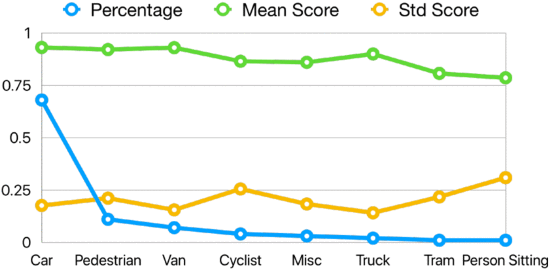
\includegraphics[width=0.8\linewidth]{images/objectnessgen.png}
\caption{Learned objectness generalization}
\end{figure}

As the number of training data decreases dramatically, the average score
tends to drops slightly and the variance tends to rise slightly. In
conclusion, the authors prove that their algorithm is guaranteed to
achieve optimality to a specific definition. On KITTI, the proposed
approach significantly outperforms past bottom-up approaches and
top-down object-based algorithms for segmenting point clouds.